\documentclass[12pt]{ORSNZ}
\usepackage{amssymb, amsmath, vmargin, graphicx, ORSNZ}
\usepackage{multirow}




\setpapersize{A4}
\setmargnohfrb{30mm}{20mm}{30mm}{20mm} % no header/footer, margins as required
\title{Partitioning of students into equitable groups using SolverStudio}
\author{M. Fairley*, O. Dowson\\Department of Engineering Science\\University of
  Auckland\\New Zealand\\{*}mfai035\@@aucklanduni.ac.nz} 

\date{} % Don't include the date
\setlength{\parindent}{6mm} % 6mm paragraph indentation
\renewcommand{\baselinestretch}{1.0417} % to get 15pt lines (does it work?)

\begin{document}

\maketitle
\pagestyle{empty} \thispagestyle{empty}
\begin{abstract}
Students in their final year of a Bachelor of Engineering at the University of Auckland are required to complete a course called `Managing a Business'. As part of this course, students are partitioned into groups of around twenty-five students and given a single week to solve a large engineering or business related problem. In order to make this partitioning equitable, the students should be partitioned in a way that makes the groups as similar as possible across several factors. These include the gender and ethnic make-up of each group, as well as the number of students from each engineering discipline and the academic performance of the students in each group. A mixed integer program was formulated to solve this problem and implemented using PuLP, SolverStudio and Excel. The model was validated against data from the 2013 cohort, and shown to improve key metrics. The end product was given to the course organiser who used the model to partition the 571 students of the 2014 class into twenty-three groups. We believe this paper provides a good case study on how the combination of Excel, SolverStudio and PuLP enables the rapid development of practical optimisation solutions.

\textbf{Key words:} excel, pulp, solverstudio, group allocator
\end{abstract}

\section{Introduction}
Students in their final year of a Bachelor of Engineering at the University of Auckland are required to complete a course known as ENGGEN403. As part of the course, students are partitioned in to groups of around 25 students and given a single week to produce a large piece of work on a given topic. In recent years, these topics have included a rebuild plan for Christchurch, a proposal for the future of Auckland’s transport network and a tender to run a new public-private partnership investment agency.

Although the stated aim of the project is to practice the skills taught throughout the course, a large component relates to team dynamics. The partitioning of students into groups has a significant impact on both group performance, and the perceived fairness amongst groups. It is of interest, to both students and staff, that the groups be both fair and equitable.

This paper details the development, implementation and results of an optimisation solution to the student partitioning problem. 

\subsection{Variables of Interest}
There is no clear definition of fair and equitable, however we can identify two distinct types of variables that are of interest: academic ability and demographic composition. The first is important as it would be unfair to have one group composed of mainly high-achieving students, and another with low-achieving students. The second is important to ensure no one feels excluded in their group, and to ensure each group has a diverse mix of people.

The variable of most interest is grade point average (GPA). A GPA is a quantitative measure of a student's academic performance. At the University of Auckland, GPA's are measured on a 1-9 scale, where 1 represents a C- average, and 9 represents an A+ average. There is anecdotal evidence from students and the course organiser of groups in previous years with large numbers of high GPA students. Although this does not necessarily lead to a better grade, there is a perception of inequity amongst students from other groups. A second cause for concern were groups with a bi-modal split of high-GPA students and low-GPA students. Therefore, two key metrics in determining the quality of any partition are the mean GPA of a group, and the variance of student GPAs within a group.

In addition, ENGGEN403 is a common paper to all the engineering disciplines at the University of Auckland. Each discipline has a unique set of skills and perspective to contribute to group projects. To give all groups an equal balance of these skills, and to prevent a single discipline from dominating a group, students from each discipline should be distributed equally amongst the groups.

Two other demographic variables are gender and ethnicity. Although these have less of an impact on group performance than GPA or discipline, group demographics can have a large impact on the perceived fairness and enjoyment by students. Therefore, there should be an equal number of students identifying as each gender in every group. Balancing on ethnicity also contributes to the perceived fairness of the groups by students.

\subsection{Previous Solution}
In previous years, the job of partitioning the students into groups has been the course organisers job. The method for doing so was not rigorous, but can be considered to be a greedy heuristic. The basic method was as follows:

Starting with the smallest discipline, distribute the students across the groups aiming to balance the mean GPA of each group. Once complete, move onto the next smallest discipline and repeat. As more students are added, try to balance gender as well as GPA. Once all students are added, perform a series of swaps between pairs of students to improve the overall balance.

This process usually took on the order of two days to complete.

\section{Mathematical model}
In this section, we define the mixed integer mathematical programme that was formulated to solve the problem.
\begin{description}
\item[Sets] \mbox{}\\
        Students: $S = \{1, 2, \dots, m\}$;\\
        Groups: $G = \{1, 2, \dots, n\}$;\\
        Ethnicities: $E = \{\mbox{P\=akeh\=a/European, M\=aori, Asian, Other}\}$;\\
        Genders: $K = \{\mbox{Male, Female}\}$;\\
        Disciplines: D = \{Civil, Chemical \& Materials, Mechatronics,Mechanical, Electrical, Software, Computer Systems, Engineering Science, Biomedical\};
        Students who identify as gender $k$: $S^K_k \subset S, \quad \forall k \in K$;\\
        Students who identify as ethnicity $e$: $S^E_e \subset S, \quad \forall e \in E$;\\
        Students who study discipline $d$: $S^D_d \subset S, \quad \forall d \in D$.



\item[Parameters] \mbox{} \\
$\gamma_s = $ grade point average of student $s$; \\
$M_g = $ the number of students in group $g$;\\
\textbf{Note:} the values of $M_g$ are computed a priori. They should add up to the total number of students in the class.\\
$\alpha = $ priority given to allocating groups with equal mean compared to groups with equal variance. This should be between 0 and 1;\\
$\beta^I = $ penalty weighting put on violating demographic constraints of type I, $I= D, E, K$;\\
$\hat{\mu} = $ mean GPA of all students;\\
$\hat{\sigma^2} = $ variance in the GPA of all students.

\item[Decision variables]\mbox{} \\
$x_{sg}\in\{0,1\} = $ 1 if student $s$ allocated to group $g$, 0 otherwise;\\
$\rho^I_{gi} = $ artificial penalty variable for group $g$, factor $i$, \qquad $I=\{K, D, E\}$;\\
$\mu_{max} = $ maximum mean GPA of any group;\\
$\mu_{min} = $ minimum mean GPA of any group;\\
$\sigma^2_{max} = $ maximum variance of GPA within any group;\\
$\sigma^2_{min} = $  minimum variance of GPA within any group.

\item[Objective Function]\mbox{} \\
The objective function is to minimise a convex combination of the spread between the maximum and minimum mean group GPA, and the spread between the maximum and minimum variance of the GPAs within a group. Adding a penalty term with a large coefficient $\beta$ is necessary as some constraints are relaxed.


\begin{equation}\begin{split}
\mbox{Minimise }&
\underbrace{\alpha\left(\frac{\mu_{max} - \mu_{min}}{\hat{\mu}}\right)}_{\mbox{normalised mean}} 
+ \underbrace{(1-\alpha)\left(\frac{\sigma^2_{max} - \sigma^2_{min}}{\hat{\sigma^2}}\right)}_{\mbox{normalised variance}}
\\&+ \underbrace{\sum_{g \in G}\left(\beta^K\sum_{k \in K}\rho^K_{gk} 
	+ \beta^D\sum_{d \in D}\rho^D_{gd} 
	+ \beta^E\sum_{e \in E}\rho^E_{ge}\right)}_{\mbox{penalty variables}}
\end{split}\end{equation}

\item[Constraints]\mbox{} \\
\textbf{Partitioning Constraint} These constraints ensure that all students are allocated to exactly one group.
\begin{equation} \label{con1}
\sum_{g=1}^n x_{sg} =  1 \qquad \mbox{$\forall s \in S$}
\end{equation}

\begin{equation} \label{con2}
\sum_{s \in S} x_{sg} =  M_g \qquad \mbox{$\forall g \in G$}
\end{equation}

\textbf{Bounds on objective variables} These constraints set the values of the variables used in the objective function.
\begin{equation} \label{minu}
\sum_{s \in S} \frac{x_{sg}\times \gamma_s}{M_g} \geq \mu_{min} \qquad \mbox{$\forall g \in G$}
\end{equation}
\begin{equation} \label{maxu}
\sum_{s \in S} \frac{x_{sg}\times \gamma_s}{M_g} \leq \mu_{max} \qquad \mbox{$\forall g \in G$}
\end{equation}

\begin{equation} \label{minv}
\sum_{s \in S} \frac{x_{sg}\times \gamma_s^2}{M_g}  - \hat{\mu}^2 \geq \sigma^2_{min} \qquad\mbox{$\forall g \in G$}
\end{equation}
\begin{equation} \label{maxv}
\sum_{s \in S} \frac{x_{sg}\times \gamma_s^2}{M_g}  - \hat{\mu}^2 \leq \sigma^2_{max} \qquad\mbox{$\forall g \in G$}
\end{equation}


\textbf{Bounds on demographic variables} These constraints set the minimum number of students in each group from each demographic sub-group. These constraints are relaxed via the addition of $\rho$ variables.
\begin{equation} \label{con3}
\sum_{s \in S^K_k} x_{sg} + \rho^K_{gk} \geq \left\lfloor\frac{M_g\times |S^K_k|}{|S|}\right\rfloor \qquad \mbox{$\forall g \in G \quad \forall k \in K$}
\end{equation}

\begin{equation} \label{con4}
\sum_{s \in S^D_d} x_{sg} + \rho^D_{gd}  \geq \left\lfloor\frac{M_g\times |S^D_d|}{|S|}\right\rfloor \qquad \mbox{$\forall g \in G \quad \forall d \in D$}
\end{equation}

\begin{equation} \label{con5}
\sum_{s \in S^E_e} x_{sg} + \rho^E_{ge}  \geq \left\lfloor\frac{M_g\times |S^E_e|}{|S|}\right\rfloor \qquad \mbox{$\forall g \in G \quad \forall e \in E$}
\end{equation}

\textbf{Variable Bounds} The allocation variables ($x$) are binary, all other variables are non-negative.
\[x_{sg} \in \{0, 1\}\]
\[\mu_{min}, \mu_{max}, \sigma^2_{min}, \sigma^2_{max}, \rho^I_{gi}  \ge 0.\]

\end{description}

\subsection{Estimating the variance of a group}
In order to calculate the variance of a population, one needs to know the square of the mean of that population. This is a non-linear function of a variable in the model. Therefore, to prevent the problem from being non-linear, we make an assumption that the mean GPA of every group is equal to the mean GPA of all the students. This changes the square from acting on a variable, to acting on a parameter. We can make this assumption as constraints (\ref{minu}) and (\ref{maxu}) act to force the mean GPA of each group towards the global mean GPA ($\hat{\mu}$).

\subsection{The affect of relaxing the demographic constraints}
It is noticed that the demographic constraints take the form of 
\begin{equation}
\sum_i x_i + y \geq z
\end{equation}
where $x_i$ and $z$ are both integer values. Since the objective is to minimise, and the objective coefficients of the $y$ variables are positive, they will optimise to their lower bound. This implies that the $y$ variables will also take integer values in an optimal solution. 

If the values are $\beta$ are large relative to the rest of the objective function, then the affect of this is to optimise the demographics of the groups first, and then proceed optimising the GPAs. When allocating small numbers of students, this is likely to lead to poor quality solutions with respect to GPA metrics. However, in ENGGEN 403 there are around 600 students every year. This means that there are likely to be multiple students with the same gender, ethnicity and discipline. Therefore, there is still enough freedom in the problem to produce a high quality solution with respect to the GPA metrics.

Any of these constraints can be removed from the model by setting the corresponding $\beta$ value to zero. This may be desirable for smaller classes where a greater emphasis is placed on GPA.

\section{Implementation}
The above model was implemented in the SolverStudio \cite{solverstudio} modelling environment (Figure \ref{FIG:solverstudio_screen}). SolverStudio is an add-in for Microsoft Excel. It acts as an interface between Excel and a variety of modelling languages including AMPL \cite{ampl}, GAMS \cite{gams}, PuLP \cite{pulp} and Gurobi \cite{gurobi}. In order to leverage the ability of SolverStudio to interface with Excel, it was decided to use the PuLP modelling language. CBC \cite{CBC} was chosen for the solver as it is the default solver for PuLP/SolverStudio.

\begin{figure}[!ht]
	\centering
	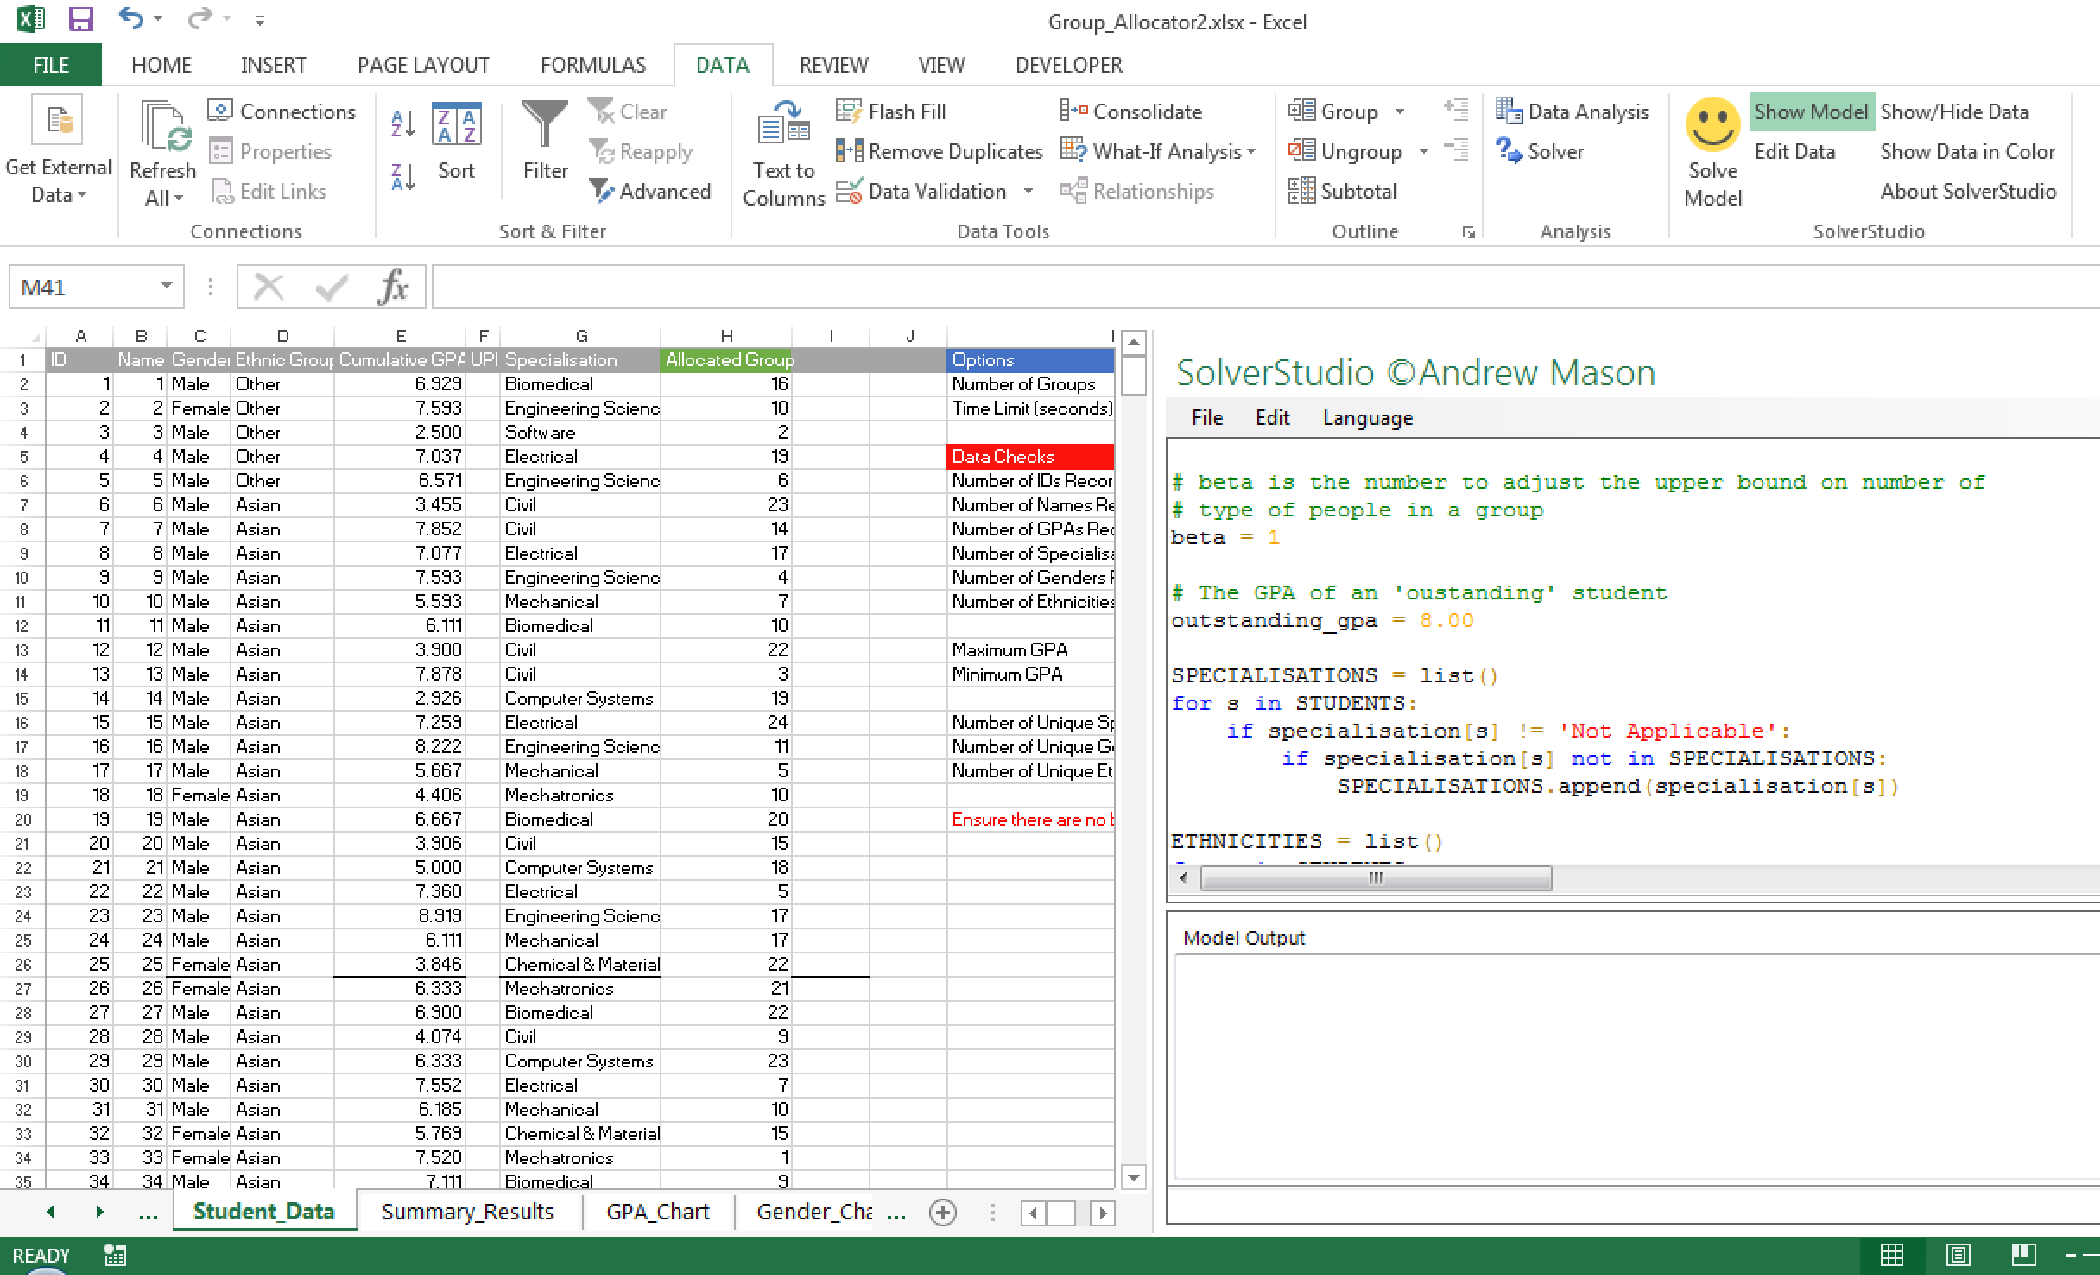
\includegraphics[width=\textwidth]{solverstudio_screenshot.pdf}
	\caption{Screenshot of the SolverStudio workbook.}
	\label{FIG:solverstudio_screen}
\end{figure}

Model data is typed into cells in Excel and \emph{named ranges} are created using SolverStudio's \emph{Edit Data} function. These ranges are dynamic, so that the user does not need to interact with this functionality. Adding a new row to the table will automatically adjust the named range in SolverStudio. This was done by using the following formula in the \emph{Cell Range} field in the SolverStudio Data Items Editor instead of hard coding a fixed range:

\begin{verbatim}
	= OFFSET(A2, 0, 0, COUNTA(A2:A10000), 1)
\end{verbatim}

where the variable being created is in column $A$ (so that the header is cell $A1$).

When the model is solved, SolverStudio loads the data from the named ranges into standard Python dictionaries that can be accessed in the usual way. This provides seamless interaction between the PuLP model object and the data. When the model has finished solving, the reverse occurs, and SolverStudio writes the solution into a named range on the sheet. In this manner, the user does not need to understand any python or optimisation modelling in order to use the programme.

Rather than solve to optimality, the user specifies a time limit for the solver.

The programme has been tested in Excel 2010 and Excel 2013 with SolverStudio version $>$0.6.x.

\subsection{Reporting} \label{reporting}
SolverStudio provides access to Excel's API (Application Programming Interface), allowing the Python code to not only create and solve the model via PuLP, but also leverage Excel's graphing functions to create a number of visualisations of the solution.

Figure \ref{FIG:solverstudio_boxplot} shows an example of one of the plots produced by the python code. In this case, boxplots of GPA are produced for each group. This enables a quick visual tool for users to understand the quality of the solution, ensuring there are no clear outliers.

\begin{figure}[!ht]
	\centering
	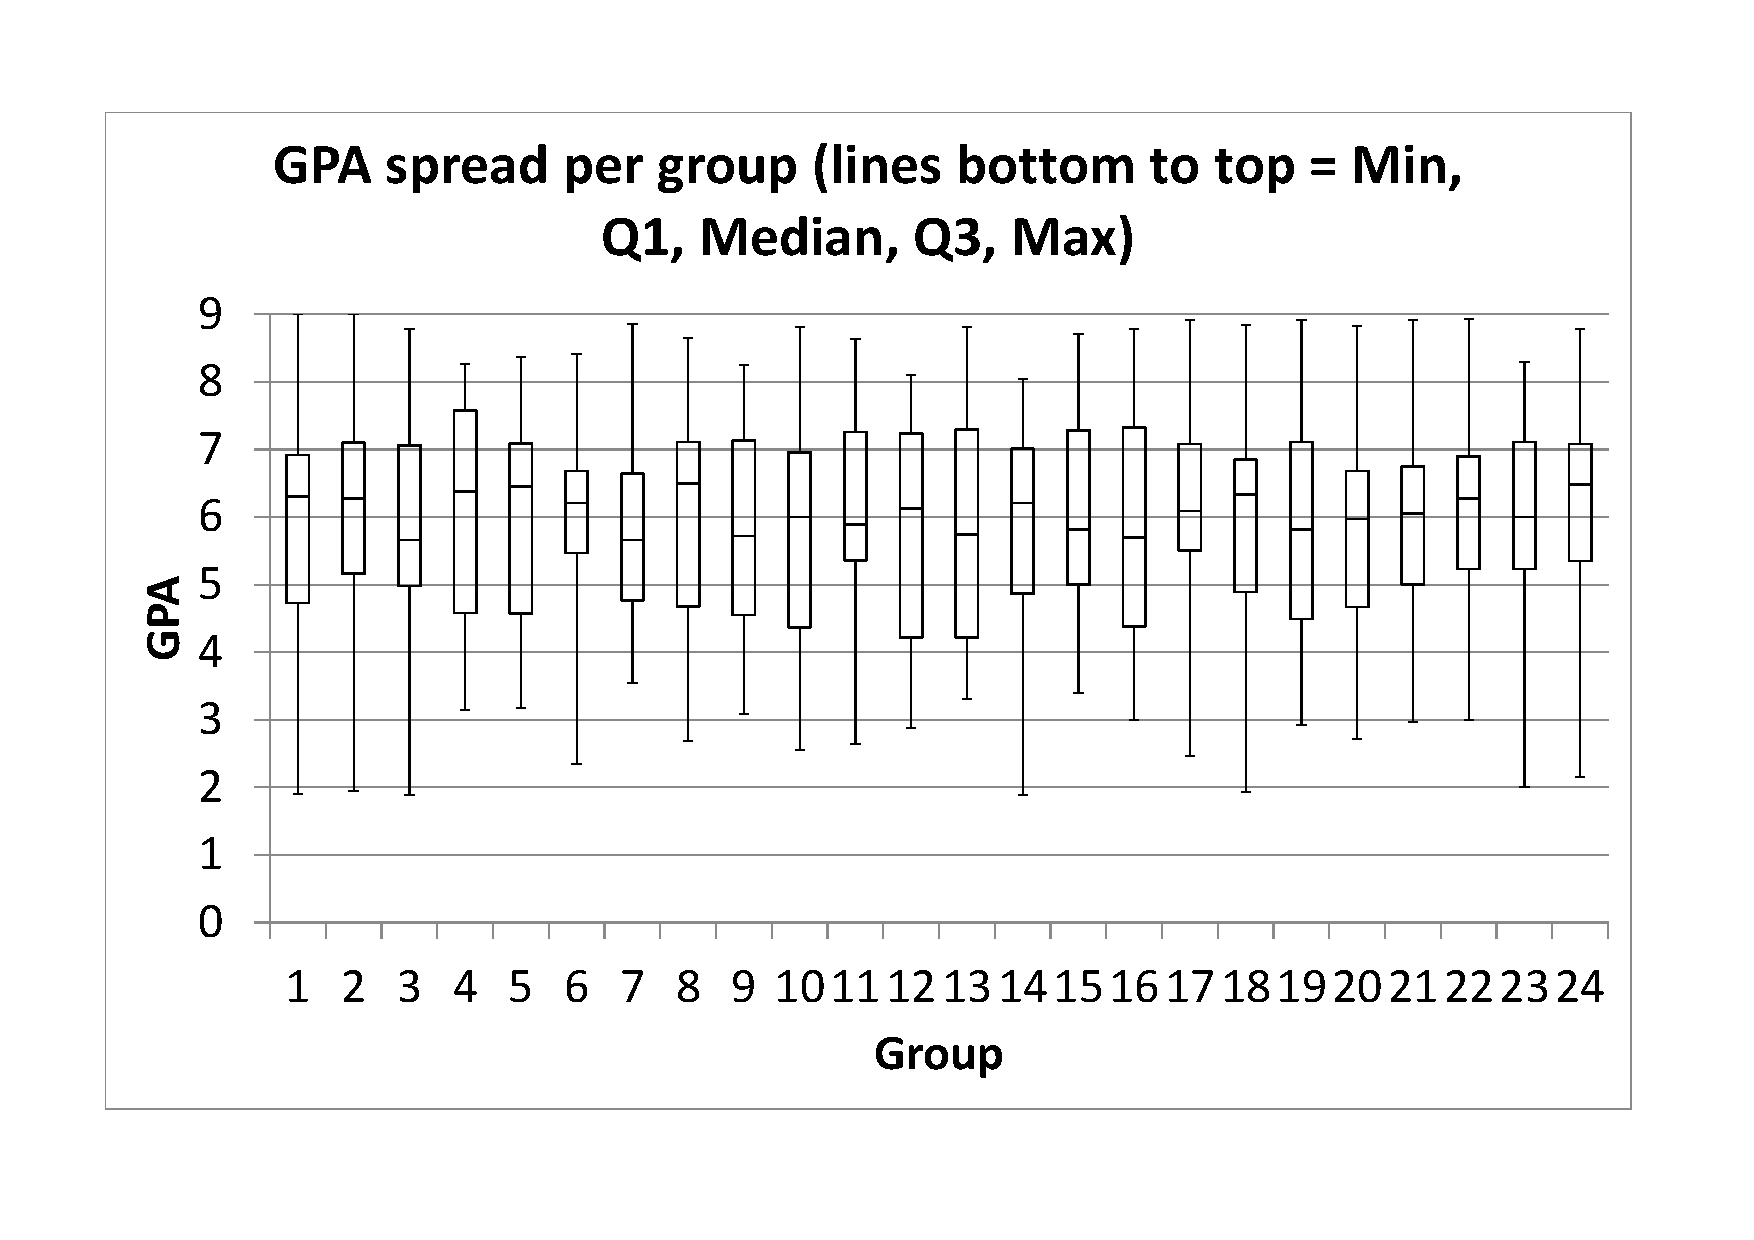
\includegraphics[trim=50 50 50 50, clip, width=\textwidth]{solverstudio_boxplot.pdf}
	\caption{Example graph produced programatically by the SolverStudio model.}
	\label{FIG:solverstudio_boxplot}
\end{figure}

In addition, Bar charts showing the number of students in each group were produced for each gender, discipline and specialisation. This allowed a visual means of checking the solution quality. 

Excel's ability to save single worksheets as a PDF (portable document format) was also utilised to create a final report that could be distributed to students showing their allocated group. This saved considerable time that was previously spent manually collating lists for students.

\section{Validation with historic data}
In 2013, 586 students enrolled in ENGGEN403. There were partitioned into 24 groups by the course organiser. To test the quality of the SolverStudio model, an anonymised version of the dataset was obtained from the course organiser.

There were 14 groups of 24 students, and 10 groups of 25 students. A value of 0.5 was used for $\alpha$, and all $\beta$ values were set to 1. The students had a mean GPA of 5.92, with a variance of 2.70. The model was solved for 120s. 

There was a small number of students who did not have a recorded discipline, or were from a different degree program. They were classified in the \emph{Other} category for discipline. 

Table \ref{TAB:results} shows the results of the partitioning for the 2013 ENGGEN403 class. The \emph{Class} column gives the corresponding value of all the students enrolled in the class. The \emph{Historic} columns give the values for the groups as allocated by the course organiser, and the \emph{SolverStudio} columns give the values for the groups created by the SolverStudio model.

Values in bold indicate that the corresponding method returned a solution with a value closer to the actual value than the alternative method.

\begin{table}[!ht]
	\centering
	\begin{tabular}{l r | c | c c | c c}
	& &  & \multicolumn{2}{c |}{Historic} & \multicolumn{2}{c}{SolverStudio}\\
	&  & Class & Min & Max & Min & Max\\[1ex]
	\hline
	& &  & \multicolumn{2}{c |}{} & \multicolumn{2}{c}{}\\[-2ex]

	\multirow{2}{*}{GPA}& Mean	&	5.92	&5.42	&6.60 	&\textbf{5.74}	&\textbf{6.05} \\
	& Variance&	2.70	&1.70	&3.83	&\textbf{2.56}	&\textbf{3.16}\\[1ex]

	\hline& &  & \multicolumn{2}{c |}{} & \multicolumn{2}{c}{}\\[-2ex]

	\multirow{10}{*}{Discipline (\%)}&Biomedical			&4.44	&4.00	&8.33	&4.00	&8.33 	\\
	&Engineering Science	&4.78	&0.00 	&8.33 	&\textbf{4.00}	&\textbf{8.00} 	\\
	&Software			&8.02	&4.00 	&\textbf{12.00}  &4.00 	&12.50 	\\
	&Electrical			&13.30 	&8.33 	&16.70 	&\textbf{12.00} 	&16.70 	\\
	&Civil				&28.70 	&25.00 	&33.30 	&\textbf{28.00} 	&\textbf{29.20} 	\\
	&Mechanical			&13.50 	&12.00 	&16.70 	&12.00	&16.70 	\\
	&Computer Systems	&6.31 	&4.00 	&12.50 	&4.00 	&\textbf{12.00} 	\\
	&Mechatronics		&9.90	&8.00 	&\textbf{12.50} 	&8.00 	&16.00 	\\
	&Chemical \& Materials&	10.60&8.00	&12.50 	&8.00	&12.50 	\\
	&Other				&0.51	&0.00	&4.17	&0.00	&4.17\\[1ex]

	\hline& &  & \multicolumn{2}{c |}{} & \multicolumn{2}{c}{}\\[-2ex]

	\multirow{2}{*}{Gender (\%)}&  Female	&26.11&	24.00&	\textbf{28.00}&	24.00&	33.33 \\
	& Male	&73.89&	\textbf{72.00}&	76.00&	66.67&	76.00 \\[1ex]

	\hline& &  & \multicolumn{2}{c |}{} & \multicolumn{2}{c}{}\\[-2ex]

	\multirow{4}{*}{Ethnicity (\%)}&	P\=akeh\=a / European	&38.57 	&25.00	&50.00	&\textbf{36.00}	&\textbf{44.00} \\
	&	M\=aori		&3.75	&0.00	&12.50	&0.00	&\textbf{8.33}  \\
	&	Asian		&53.75	&41.67	&64.00	&\textbf{52.00}	&\textbf{58.33} \\
	&	Other		&3.92	&0.00	&8.33	&0.00	&8.33

	\end{tabular}
	\caption{Partitioned composition of the 2013 ENGGEN 403 class.}
	\label{TAB:results}
\end{table}

\subsection{Grade Point Average}

\begin{figure}[!ht]
	\centering
	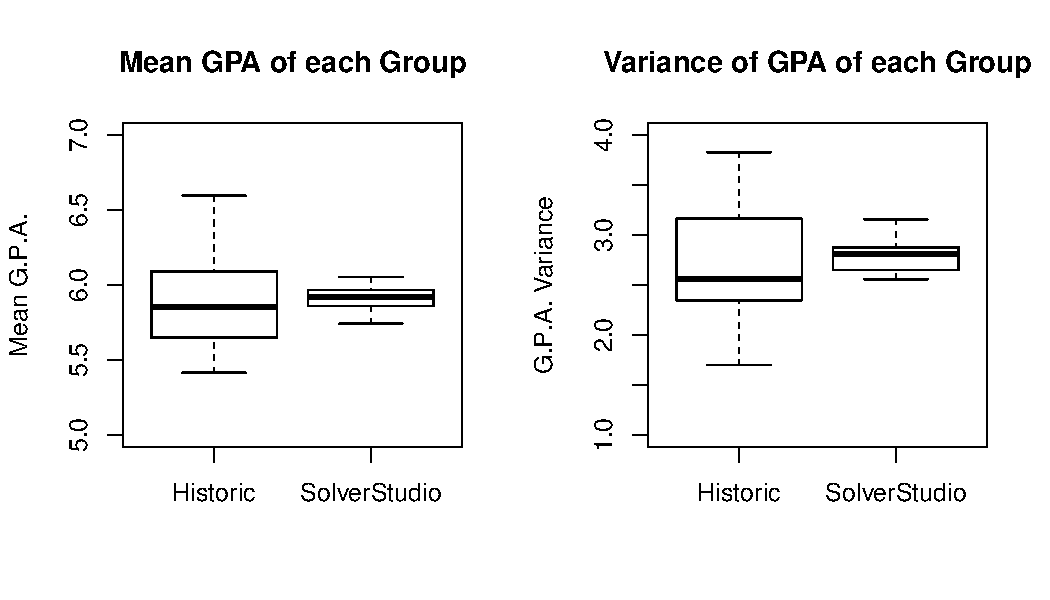
\includegraphics[width=\textwidth]{./gpa_plot.pdf}
	\caption{Boxplots of mean group GPA and variance within group GPA for historic and optimisation partitionings.}
	\label{FIG:boxplots}
\end{figure}

When compared to the 2013 partitioning, the SolverStudio partitioning reduces the spread in mean GPA between the groups. The lowest mean GPA of any of the groups is 5.74 (compared to 5.42 for the historic solution), while the highest mean GPA is 6.05 (compared to 6.6 for the historic solution). 

Similarly, the SolverStudio model created groups with a larger minimum GPA variance (2.56 compared to 1.7), and a smaller maximum GPA variance (3.16 compared to 3.83) than the historic partitioning.

This improvement can also be seen visually in boxplots of the mean and variance of the GPAs of each group (Figure \ref{FIG:boxplots}). In both cases the SolverStudio solution has a smaller spread than the historic solution, resulting in more similar groups.

\subsection{Discipline}
When compared to the historic partitioning, the SolverStudio partition performed better in six metrics and poorer in two metrics. The historic partitioning had a smaller maximum number of software students (12\% compared to 12.5\%) and a smaller maximum number of Mechatronics students (12.5\% compared to 16\%). 

In addition, there was one group in the historic partitioning with zero Engineering Science students. In the SolverStudio solution there were at minimum 4\% Engineering Science students.

\subsection{Gender}
When compared to the historic partitioning, the SolverStudio solution created a poorer partitioning of students based on gender. There was at most 28\% females in a group in the historic partitioning compared to 33.3\% in the SolverStudio partitioning. There was a corresponding difference in the minimum percentage of male students.

\subsection{Ethnicity}

The SolverStudio partitioning has both a higher minimum number of students and a smaller maximum number of students.

\section{Discussion}
This paper provides a case study on how the combination of Excel, SolverStudio and PuLP enables the rapid development of non-trivial optimisation solutions. The total development timeframe, from conception to delivery of a finished product, took two weeks of part time work. The majority of this was spent creating the reporting and visualisation tools. Using this model as a guide for future problems will reduce this time even further.

Due to the difficulty in obtaining historic data, and partitioning students manually, there was only one dataset with which to compare the SolverStudio model to historic solutions. Nevertheless, the SolverStudio model was demonstrated to improve GPA distribution of students, whilst maintaining or improving demographic distribution in a significantly shorter amount of time.

Although the SolverStudio solution improved almost all metrics than when compared to the historic solution, it resulted in a poorer partitioning with respect to gender. The likely reason for this is that the course organiser placed more emphasis on balancing gender than other demographic factors. This could be overcome in future by the $B^K$ value. This small decrease in gender equity between groups is offset by the more even distributions of students by discipline and ethnicity.

One issue with the model was that it took a long time to solve to optimality. This is due to a variety of factors, but chiefly the large number of binary variables (number of students $\times$ number of groups). Although the CBC solver quickly (less than one minute) finds a good integer solution, it is unable to find an optimal solution. 

% One reason for this is that the solution to the relaxed problem has the trivial solution where a fraction of each student of each student is allocated to each group, enabling a perfectly balanced partition. This creates a large bound gap (the distance between the relaxed problem and the optimal integer solution) for the solver to overcome.

% \emph{Another reason is the nature of the binary variables. A branch and bound approach is inefficient at increasing the lower bound at it requires near complete enumeration of the branch and bound tree (?).}


Other approaches, such as a set partitioning formulation, may improve the solution time and quality. However, given that students are unaware of the GPAs of other students in their groups, they are unlikely to perceive a small improvement in solution quality. It was for this reason, and the tight development timeframe, that other approaches were not investigated.

This case study also highlights the ability for SolverStudio to abstract a large amount of complexity from the end user. The course co-ordinator needed only minutes of instruction to be able to successfully use the spreadsheet without supervision. Where the task of partitioning the students previously took two days, the Excel spreadsheet is able to achieve a more equitable result in the time it takes to make a cup of coffee.

Optimisation does not always need to be applied to large commercial problems to be beneficial. Instead, there exist a large number of problems where years of experience has culminated in a solution that is `good enough'. Simple solutions to these problems can be created using SolverStudio in a short span of time that are user friendly and significantly reduce the work required by the user, freeing then up for more productive activities.

\section*{Acknowledgments}
The authors gratefully acknowledge Dr. Keith Adams of the Civil Engineering Department at the University of Auckland for providing valuable feedback, as well as the historical data used to validate the model. The final spreadsheet can be found on GitHub at http://www.github.com/odow/group-allocator.

\bibliographystyle{achicago}
\bibliography{ORSNZ}

\end{document}
